
\begin{frame}{Древовидная структура хранения файлов.}
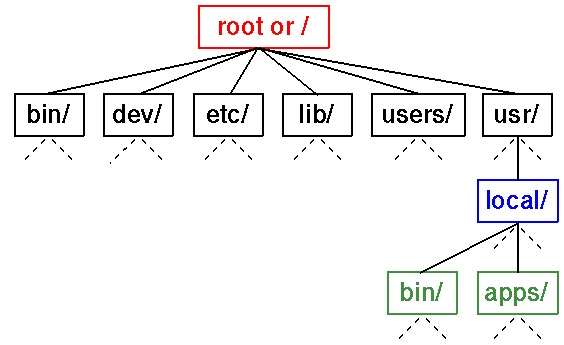
\includegraphics[height=4cm]{unix_tree} 
  \begin{itemize}
    \item Каждый файл имеет \alert{имя}, определяющее его расположение в дереве FS.
    \item \alert{Директория} объект в файловой системе позволяющий группировать файлы и другие директории.
  \end{itemize}
\end{frame}

\begin{frame}[fragile]{Относительный и полный путь к файлу.}
 Для каждой запущенной программы в системе определена \alert{текущая директория} 
 (working directory or current working directory) 
  \begin{itemize}
    \item \alert{относительный путь} - от текущей директории \newline
      Примеры имен: ../user10/.bashrc; ./script; script \newline
        \alert{./} - текущая директория \newline 
        \alert{../} - предыдущая директория \newline 
        \alert{../../} - две предыдущих директории 
    \item \alert{полный путь} начинается с \alert{/}(корневой директории), 
    \item директории разделяются символом \alert{/}. \newline
  \end{itemize}
\end{frame}


\begin{frame}{Абсолютное имя файла в дереве файловой системы.}
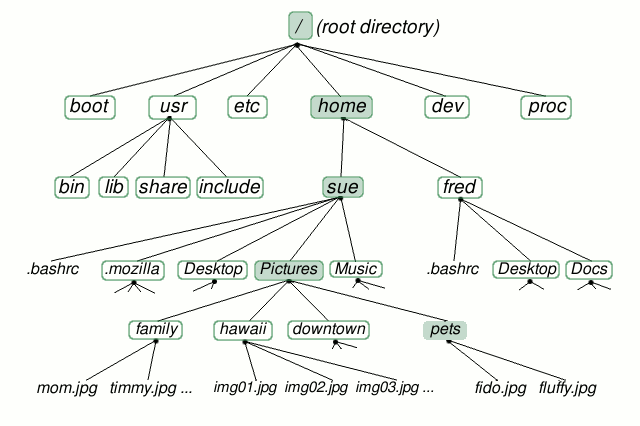
\includegraphics[height=8cm]{filesystem} 
\end{frame}

%\begin{frame}{Примеры использования имен.}
%        /proc/cmdline
%
%        /boot/grub/grub.cfg
%
%        /home/user/.ssh/authorized\_key \newline 
%\end{frame}

\begin{frame}[fragile]{Перемещение по файловой системе}
      \begin{itemize}
      \item {\tt pwd} -- имя текущей директории (help pwd)
      \item {\tt realpath ./}
		  \item {\tt ls} -- список файлов в директории. По умолчанию в текущей (man ls)
		  \item {\tt cd} -- смена текущей директории (help cd)
      \end{itemize}
      \begin{block}{Упражнение. Заходим в /usr/bin/ и просматриваем список доступных команд.}
\begin{lstlisting}
pwd
cd /usr/bin/
pwd
ls
cd -
pwd
\end{lstlisting}
      \end{block}
\end{frame}


%\begin{frame}[fragile]{Просмотр типов файлов}
%      \begin{block}{Упражнение. Символьное обозначение типа файла.}
%Первая буква вывода команды ls -l обозначает тип файла. 
%Tip. Команды file позволяет определить тип файла. Ключ -d для работы с
%директорией. 
%
%/dev/zero
%
%/dev/sda 
%
%.. 
%
%/bin/sh 
%
%/dev/log
%
%/dev/stdout
%      \end{block}
%\end{frame}

\begin{frame}{Типы файлов в Unix}
  Для пользователя:
  \begin{itemize}
    \item \alert{Обычные файлы (regular file)}: .bashrc, /bin/bash
    \item \alert{Каталоги (directory)}: /home/user1, /usr, /, /usr/local  \pause
    \item \alert{Символические ссылки (symbolic links)}: /bin/sh, /dev/stdout
  \end{itemize} \pause
  Для администратора:
  \begin{itemize}
    \item \alert{Файлы устройств (device special file)}:
      \begin{itemize}
        \item \alert{блочные}: /dev/sda5, /dev/loop0, /dev/sr0
        \item \alert{символьные}: /dev/null, /dev/mem, /dev/tty
      \end{itemize}
  \end{itemize} \pause
  Для программиста:
  \begin{itemize}
    \item \alert{FIFO (named pipe)}: /dev/xconsole
    \item \alert{Socket}: /dev/log
  \end{itemize}

\end{frame}

%\begin{frame}[fragile]{Создание (текстовых) файлов}
%  \pause
%  \begin{enumerate}
%    \item Любимым редактором: \alert{vi/vim}, \alert{nano}, \alert{mcedit} \pause
%    \item \alert{echo}
%\begin{lstlisting}
%echo какой-то текст >file
%\end{lstlisting}\pause
%    \item \alert{cat} с перенаправлением\footnote{До ``конца ввода'', т.е. нажатия Ctrl+D}
%\lstinputlisting[basicstyle=\small]{../../sam-solutions/samples/cat-input-file} \pause
%    \item \alert{touch} - создать пустой файл
%\begin{lstlisting}
%~$ touch file4
%~$
%\end{lstlisting}
%  \end{enumerate}
%\end{frame}
%

%\begin{frame}[fragile]{Особенности именования файлов.}
%
%                \begin{itemize}
%                    \item case sensitive \alert{fileA} и \alert{Filea} - два разных имени
%                    \item один файл может иметь \alert{несколько} имен (hardlink) 
%                    \item \alert{/} разделяет директории. Не получиться присвоить.
%                    \item \alert{.}file - скрытый файл. По умолчанию пропускаются.
%                    \item максимальная длина имени \alert{255} символов
%                \end{itemize}
%\end{frame}

\begin{frame}[fragile]{Команды для работы с файлами}
Any ideas what is purpose of this commands? 
	\begin{itemize}
		\begin{columns}
		\column{0.2\textwidth}
			\item cp
			\item mv
			\item rm
			\item file
		\column{0.2\textwidth}
			\item touch
			\item ln
			\item mkdir
%			\item mknod
%			\item mkfifo
		\end{columns}
	\end{itemize}
\end{frame}


\begin{frame}[fragile]{Операции над каталогами (и файлами)}
  \begin{itemize}
    \item \alert{mkdir} - создать каталог
\begin{lstlisting}
~$ mkdir dir1 /tmp/somedir
~$ mkdir -p dir/and/existant/parts/in/path
\end{lstlisting} \pause
%    \item \alert{rmdir} - удалить (пустой) каталог
%\begin{lstlisting}
%~$ rmdir dir1 /tmp/somedir
%~$ rmdir -p deep/empty/dir/structure/
%\end{lstlisting} \pause
    \item \alert{cp} - копирование файлов\footnotemark[8]
    \item \alert{mv} - перемещение и переименование файлов
    \item \alert{rm} - удаление файлов\footnotemark[17]
\begin{lstlisting}
~$ rm -rf dir1 /tmp/somedir
~$ cp /etc/passwd /tmp/passwd # copy file to file 
~$ cp -r /etc/  /tmp/ # copy directory to directory
\end{lstlisting}
  \end{itemize}
\footnotetext[8]{с ключом \alert{-r}) и каталогов}
\end{frame}
